\section{Task graph}
\label{sec:taskgraph}

This section documents how the HII search is wired into \swift's task
graph, focused on the stellar/radiation part only (not hydro or
gravity, except where radiation depends on them). Source-line
references below point to specific lines in the current
implementation; identifiers (function and variable names), not line
numbers, are the stable anchor if the code shifts.

\subsection{Why this is not a regular self/pair task}
\label{sec:not-regular}

An ordinary \swift self/pair loop (e.g.\ hydro density) is created once
per pair of neighbouring cells at \code{hydro.super}, and
\code{scheduler\_splittasks} recursively breaks each one into many
independent, finer self/pair tasks wherever
\code{cell\_can\_split\_self/pair\_hydro\_task} says the cut-off
radius still fits inside a sub-cell: so the actual density/force
calculation is spread across potentially hundreds of small,
independently-schedulable tasks that each touch only two specific
cells.

The radiation search does not work this way, for two reasons: (1) the
relevant length scale, $h_{\rm hii}$, is not a fixed smoothing length
but a search radius that grows dynamically over many rebuild cycles,
so no single tree level is guaranteed to contain it; and (2) the
consumption logic is inherently sequential and global to one star (a
star's photon budget must be spent in strict distance order across
\emph{all} its candidates, not independently per cell-pair). So the
implementation splits the work into two different kinds of task:

\begin{itemize}
  \item \textbf{\code{task\_subtype\_stars\_radiation\_in} /
    \code{\_out}} (self and pair): created once at the
    \emph{top-level} cell grid (27-neighbour stencil,
    \code{engine\_make\_radiationloop\_tasks\_mapper},
    \code{engine\_maketasks.c:4250}), \textbf{as implicit tasks}
    (\code{implicit=1} in \code{scheduler\_addtask}): they run no
    compute code at all (no case for them in \code{runner\_main.c}'s
    dispatch switch). Their only job is to exist as dependency nodes:
    every drift/sort/cooling task that must finish before the search
    reads that region unlocks the matching \code{\_in} task; the
    \code{\_out} task unlocks \code{stars\_out} once the search is
    done. They are never split further by
    \code{scheduler\_splittasks}.
  \item \textbf{\code{task\_type\_stars\_hii\_ionization\_feedback}}
    (subtype \code{none}): a \emph{single, coarse-grained} task
    created once per \code{radiation\_level} cell
    (\code{engine\_make\_hierarchical\_tasks\_radiation\_subgrid},
    \code{engine\_maketasks.c:2110}). This is the only task that
    actually runs code (\code{runner\_do\_stars\_hii\_\allowbreak
    ionization\_feedback}, dispatched at \code{runner\_main.c:582}).
    It performs its own manual, run-time recursion down to the
    ``Working Level'' and its own per-star neighbour search internally;
    see Section~\ref{sec:runtime}. From the scheduler's point of
    view this is one big task per region, not many small ones.
\end{itemize}

\subsection{\texttt{radiation\_level}: a coarsening criterion decoupled from \texttt{hydro.super}}

\code{cell\_can\_split\_pair\_radiation\_subgrid\_task} /
\code{cell\_can\_split\_self\_radiation\_subgrid\_task}
(\code{cell.h:1276}, \code{1332}) are radiation's own splitting
criteria, structurally identical to the hydro ones but with an extra
term: a cell stops splitting (and \code{radiation\_level} is pinned
there) once
\begin{equation}
  \text{space\_stretch} \times \gamma_{\rm kernel} \times h_{{\rm hii},\max} \ge 0.5\, d_{\min},
\end{equation}
\emph{in addition to} the ordinary hydro/star/sink/BH $h_{\max}$
terms, and also \texttt{c->hydro.super\allowbreak{} == NULL} (i.e.\ radiation never
splits finer than \code{hydro.super}, only coarser). Since $h_{\rm
hii}$ can grow far beyond an ordinary smoothing length as a star's
search radius expands, \code{radiation\_level} can sit strictly
\emph{above} \code{hydro.super}: one radiation task then covers
several \code{hydro.super} subtrees at once. When $h_{\rm hii}$ is
small this term is inert and
\texttt{radiation\_level\allowbreak{} == hydro.super} for free. \code{cell\_set\_super\_radiation\_subgrid}
(\code{cell.c:1368}) walks the tree and stamps
\code{c->stars.radiation\_level} to the shallowest ancestor holding
a \code{radiation\_in} link.

\textbf{Why an orphaned link cannot occur.} The run-time search
(\code{runner\_dosub\_stars\_hii\_ionization\_feedback}) only ever
reads \code{radiation\_level}'s \emph{own} link list, never descends
into its children's links: if a cell held its own \code{radiation\_in}
link while an ancestor was stamped as \code{radiation\_level} instead
(e.g.\ from two neighbouring regions with \code{hydro.super} at
different depths, as non-uniform density can produce), that link would
become permanently invisible to the flat walk, a silent
search-incompleteness bug rather than a crash. This is prevented by
construction: \code{scheduler\_splittask\_radiation\_subgrid}
(\code{src/scheduler\_splittasks.c}) splits a radiation pair
\emph{asymmetrically} whenever only one side can still descend,
enumerating that side's facing progeny geometrically against the
other, coarser side rather than forcing both to a shared depth, so
each cell always settles at its \emph{own} \code{radiation\_level} and
never leaves a link stranded above it. A \code{SWIFT\_DEBUG\_CHECKS}
assertion (\code{cell.c:1393}) is kept as a live regression tripwire
for this invariant.

\subsection{Dependency wiring}

For every \code{radiation\_in} self/pair task \code{t} covering
cell(s) \code{ci}/\code{cj}, \code{engine\_\allowbreak
make\_extra\_radiationloop\_tasks\_mapper}
(\code{engine\_maketasks.c:3636}) creates the matching
\code{radiation\_out} task and wires, via
\code{engine\_radiation\_wire\_super\_deps}
(\code{engine\_maketasks.c:3572}, which recurses down to every
\code{hydro.super} beneath a coarse \code{radiation\_level} cell,
visiting each disjoint subtree exactly once), the dependency chain
shown in Figure~\ref{fig:dep-chain}: for every \code{hydro.super}
beneath $ci$/$cj$, its own drift/sort/cooling/feedback-ghost tasks all
unlock \code{radiation\_in}, which feeds the single coarse-cell
computation, which unlocks \code{radiation\_out}, which unlocks
\code{stars\_out} on every \code{hydro.super} beneath $ci$/$cj$ (and,
once, \code{timestep\_sync} at the main \code{super}, if that policy
is active).

\begin{figure}[h]
  \centering
  \begin{tikzpicture}[
      font=\small,
      node distance=6mm,
      pre/.style={rectangle, draw, minimum width=6.4cm, align=center, fill=black!4},
      imp/.style={rectangle, draw, dashed, minimum width=6.4cm, align=center},
      comp/.style={rectangle, draw, thick, minimum width=6.4cm, align=center, fill=black!12},
    ]
    \node[pre] (pre) {per \code{hydro.super} beneath $ci$/$cj$:\\
      \code{drift\_hydro}, \code{sorts\_hydro}, \code{cooling\_out},\\
      \code{drift\_stars}, \code{feedback\_ghost}};
    \node[imp, below=of pre] (rin) {\code{radiation\_in} \scriptsize(implicit, no compute)};
    \node[comp, below=of rin] (hii) {\code{hii\_ionization\_feedback} \scriptsize(the only task that runs code)};
    \node[imp, below=of hii] (rout) {\code{radiation\_out} \scriptsize(implicit, no compute)};
    \node[pre, below=of rout] (sout) {\code{stars\_out} \scriptsize(per \code{hydro.super} beneath $ci$/$cj$)};
    \node[imp, below=of sout] (tsync) {\code{timestep\_sync} \scriptsize(once, main \code{super}, if policy active)};
    \draw[->] (pre) -- (rin);
    \draw[->] (rin) -- (hii);
    \draw[->] (hii) -- (rout);
    \draw[->] (rout) -- (sout);
    \draw[->, dashed] (sout) -- (tsync);
  \end{tikzpicture}
  \caption{Dependency chain wired by
    \texttt{engine\_radiation\_wire\_super\_deps}, restricted to the
    stellar/radiation tasks (hydro/gravity tasks outside this chain
    are omitted). Shaded/thick box: the one task that actually runs
    compute code. Dashed boxes: implicit barrier tasks, dependency
    nodes only. This is a schematic of the chain described in the text,
    not an automated dump of the runtime task graph.}
  \label{fig:dep-chain}
\end{figure}

A \code{SWIFT\_DEBUG\_CHECKS} invariant enforces that a
\code{radiation\_in} pair task always connects two \emph{distinct}
\code{radiation\_level} regions (\code{engine\_maketasks.c:3722}):
otherwise both sides would wire identical unlocks onto the same
\code{hii\_ionization\_feedback} task, a duplicate-unlock error.

\subsection{Activation (unskip)}
\label{sec:unskip}

\code{cell\_unskip\_radiation\_tasks} (\code{cell\_unskip.c:2273})
walks \code{c->stars.radiation\_in} and \code{radiation\_out}
each timestep. For every active task it also activates
drift/sync/\code{stars\_in} (or \code{stars\_out}) over
\emph{every} \code{hydro.super} beneath the possibly-coarse
\code{radiation\_level} cell(s)
(\code{cell\_radiation\_activate\_supers\_in/out}, factored out
specifically because a single \code{c->hydro.super} dereference
would be NULL or wrong for a coarsened region). The pair branch also
runs the radiation-specific rebuild check,
\code{cell\_need\_rebuild\_for\_radiation\_pair}: the ordinary
\code{cell\_need\_rebuild\_for\_stars\_pair} is blind to $h_{\rm
hii}$ growth between rebuilds and would under-trigger.
\code{c->stars.hii\_ionization\_feedback} itself is unskipped
unconditionally alongside the other per-cell tasks
(\code{cell\_unskip.c:2807}) whenever the cell needs activating.

\subsection{Locking}

\code{hii\_ionization\_feedback}'s search reads and writes gas across
\code{ci}'s own subtree plus every neighbouring region reachable
through \code{ci->stars.radiation\_in} (\code{task.c:808}, lock;
\code{task.c:577}, unlock). Locking proceeds in
\code{radiation\_in}'s link order: \code{ci}'s own star and hydro
trees first, then each linked pair task's ``other'' cell's hydro tree
(locking a region's tree also blocks its descendants/ancestors via
\code{cell\_locktree}'s hold-counter, so one lock per neighbouring
region suffices: no need to enumerate every \code{hydro.super}
beneath it individually). If any lock in the chain fails, everything
already acquired for this task is rolled back and the task is
requeued: same contention pattern as any other two-cell pair lock,
not a novel risk, but link order is only locally (not globally)
consistent across two regions locking each other, so genuine
lock-order contention between neighbours is possible under load.

\subsection{Run-time recursion and neighbour search}
\label{sec:runtime}

Once \code{hii\_ionization\_feedback} actually runs
(\code{runner\_do\_stars\_hii\_ionization\_feedback},
\code{runner\_radiation\_feedback.c:259}), it manually recurses down
\code{c->progeny} (mirroring what \code{scheduler\_splittasks}
would have done for an ordinary task, but at run time inside a single
task) until it reaches the ``Working Level'': a cell no smaller than
needed to contain the current interaction limit: then hands off to
\code{runner\_dosub\_stars\_hii\_ionization\_feedback}
(\code{runner\_radiation\_feedback.c:471}).

\begin{figure}[h]
  \centering
  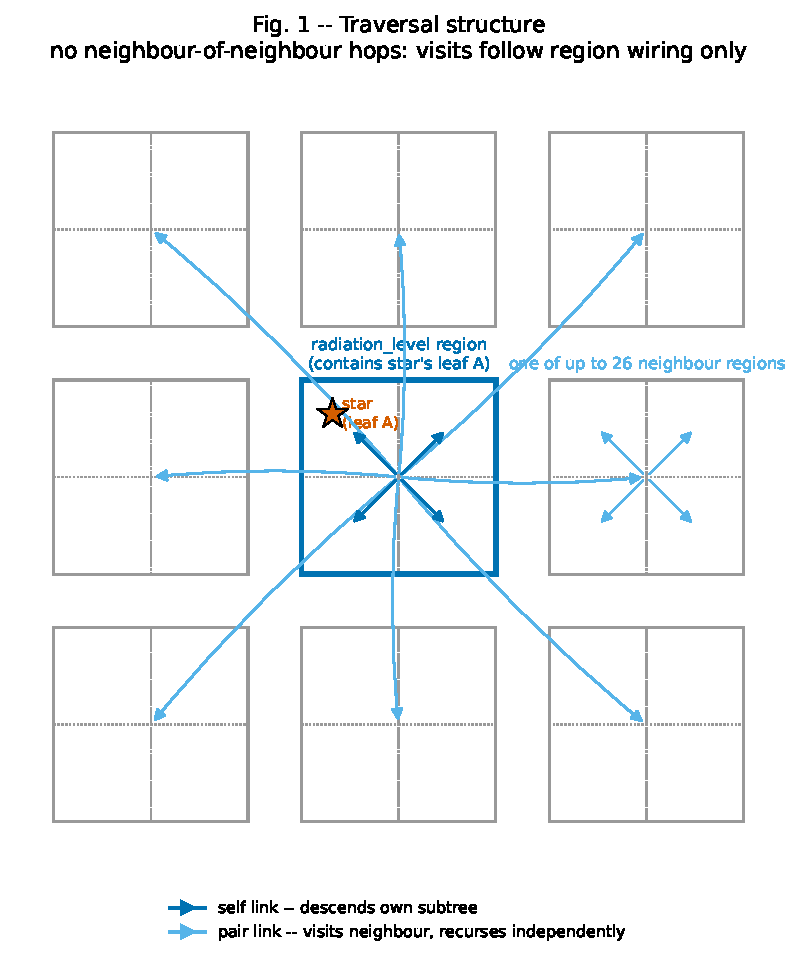
\includegraphics[width=0.75\linewidth]{figures/fig1_traversal_structure.pdf}
  \caption{Star-centric traversal from a \texttt{radiation\_level} cell:
    the self link descends the star's own region, and each pair link
    descends one of up to 26 neighbour regions. There are no
    neighbour-of-neighbour hops: every cell the search visits is
    reached directly from \texttt{radiation\_level}'s own link list.}
  \label{fig:traversal-structure}
\end{figure}

For each active star at that level:
\begin{enumerate}
  \item Gather candidates within the current search radius via
    \code{runner\_do(self/dopair)\_stars\_hii\_ionization\_feedback},
    walking \code{c}'s own cell and every cell reachable through
    \code{c->stars.radiation\_level->stars.radiation\_in} (the same
    link list used for locking/dependencies) into a fixed-size,
    distance-sorted buffer (\code{max\_ngbs}), filtered by
    \code{feedback\_part\_can\_be\_ionized} (not already tagged, cold
    enough, dense enough) and, if angular splitting is on, by whether
    the candidate's assigned pixel still has budget. When the search
    radius spans several wired leaf cells, each is tested
    independently and its candidates merge into this one global,
    distance-sorted buffer (Fig.~\ref{fig:multi-leaf-merge}), so
    ``closest-first'' in step 2 below means closest across the whole
    search, not just within one leaf.
  \item Consume the star's budget on the sorted buffer, closest first
    (Eq.~\ref{eq:recomb-cost}), applying the deterministic/probabilistic
    boundary-particle rule at exhaustion.
  \item Retry: if the buffer filled up (more candidates may exist at
    the \emph{same} radius, just bumped out by the buffer's size cap),
    retry at the same radius, up to
    \code{Stars:HII\_max\_retry\_full\_buffer} times, but only if the
    attempt that just ran claimed at least one candidate anywhere. A
    same-radius retry re-runs the identical search over the identical
    eligible set, meets the identical per-pixel budgets, and draws the
    identical fixed (star, pixel, \code{ti\_begin}) random number
    (Section~\ref{sec:angular-splitting} of the algorithm document) at
    every pixel: if the previous attempt claimed nothing, none of
    these three inputs changed, so a retry is provably a no-op, and
    the loop exits immediately rather than repeating it up to the
    configured retry count. If the buffer did \emph{not} fill up but
    budget remains, the radius itself is the bottleneck: expand it
    by \code{Stars:HII\_radius\_expansion\_factor}, up to
    \code{Stars:HII\_max\_radius\_expansion\_tries} times, bounded by
    \code{Stars:HII\_max\_search\_radius}. These two retry kinds are
    genuinely different failure modes and must not be conflated (see
    the comment at \code{runner\_radiation\_feedback.c:613}); the
    loop breaks once the budget is exhausted or both retry budgets run
    out.
\end{enumerate}

\begin{figure}[h]
  \centering
  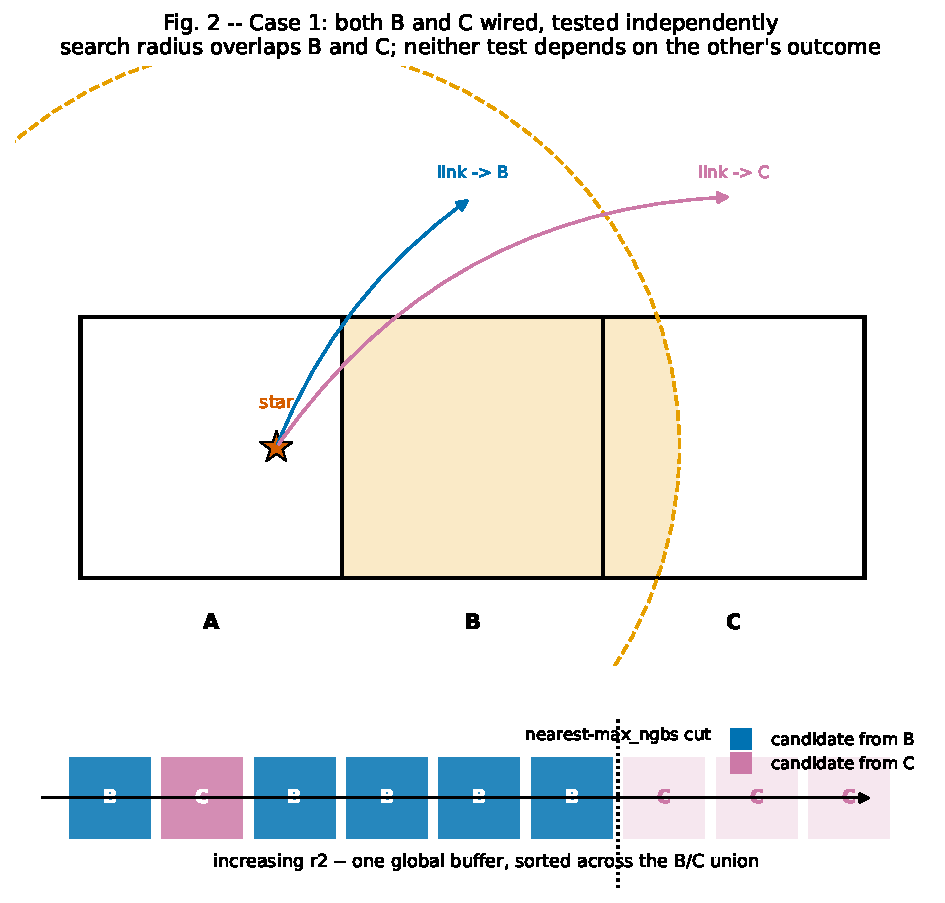
\includegraphics[width=0.85\linewidth]{figures/fig2_case1_independent_merge.pdf}
  \caption{Step 1's multi-leaf gather: a search radius covering several
    wired leaf cells tests each independently, then merges their
    candidates into one global nearest-\texttt{max\_ngbs} buffer.}
  \label{fig:multi-leaf-merge}
\end{figure}

This retry/expansion loop, not \code{scheduler\_splittasks}, is what
makes the search radius-adaptive: it is why hitting
\code{Stars:HII\_max\_search\_radius} (the GEAR radiation logbook's
Validation section)
shows up as the search radius simply never being allowed to expand past
the configured ceiling, not as a scheduler-level task-graph error.

\textbf{Expansion probes can outrun the coherent front.} Each radius
expansion searches a strictly larger volume for the \emph{same} pixel
budget. At \code{HII\_angular\_nside}$\,\ge1$, a cone whose remaining
budget is already small relative to a single particle's cost can still
win its probabilistic boundary draw on a candidate found only after
several expansions: well outside the volume that cone has actually
been paying to keep ionized. The result is an isolated tagged particle
beyond the coherent ionization front: bounded (Eq.~\ref{eq:budget-open}
of the algorithm document caps the overdraft at one particle's cost)
and accepted, not a task-graph defect: the search itself is bounded
by \code{max\_reachable\_search\_radius}
(Section~\ref{sec:sorted-gather}) and
\code{Stars:HII\_max\_search\_radius}, so the artifact cannot grow
without limit. The historical-extent front-radius measure used to read
out this model's ionized region (Section~\ref{sec:front-radius} of the
algorithm document) is specifically robust to it: an isolated particle
tagged this way is exactly the gap-separated outlier that measure's
rejection removes.

\textbf{Gather-time pixel-budget starvation guard.} Without the
per-candidate pixel-budget filter in step 1 above, a dense clump in one
pixel's direction could exceed the buffer's capacity on its own,
permanently monopolizing it: that pixel's own budget exhausts quickly,
but its now-dead candidates keep re-winning the nearest-distance
ranking on every retry, burning out
\code{HII\_max\_retry\_full\_buffer} re-finding the same dead pixel
before the search ever reaches radius expansion: leaving a sparse
pixel's budget completely unspent. All four
\code{runner\_hii\_buffer\_insert} call sites (self, dopair-naive, and
both branches of the sorted dopair) gate the insert on
\code{feedback\_get\_star\_ionization\_rate(si, pixel) > 0.0}, so a
pixel with an exhausted budget can no longer monopolize buffer slots on
retry. A milder residual (two live
pixels, one much denser, slowing rather than deadlocking the sparse
one's service rate) remains deliberately unaddressed: would need
per-pixel bounded buffer segments to fix robustly, only worth building
if a clumpy test shows it matters in practice.

\subsection{Sorted gather mechanics: one-sided scans on a global axis}
\label{sec:sorted-gather}

Within each unsplit receiver cell reached by the traversal of
Section~\ref{sec:runtime}, the gather may use that cell's hydro sort
arrays as a pre-filter
(\code{runner\_dopair\_stars\_hii\_ionization\_feedback}). The way it
does so differs structurally from the classic two-sided hydro
\code{DOPAIR}, and the difference is what frees the search from any
adjacency requirement between the star's cell and the receiver
(Fig.~\ref{fig:dopair-contrast}).

\textbf{Sort entries live on a global axis.} A cell's sort entry along
axis \code{sid} is the particle's \emph{absolute} position projected
onto the unit vector \code{runner\_shift[sid]}
(\code{runner\_do\_hydro\_sort}, \code{src/runner\_sort.c}): a
coordinate on a global 1D axis, computed with no reference to any
partner cell. The gather projects the star onto that \emph{same} axis,
$d_{i,\star} = (\vec{x}_\star - \vec{s})\cdot\hat{e}_{\rm sid}$, where
$\vec{s}$ is purely the periodic-wrap shift (zero for a non-wrapped
pair). The receiver's sorted list is then scanned only inside the window
$[d_{i,\star} - R - \Delta,\; d_{i,\star} + R + \Delta]$, with $R$ the
current search radius and $\Delta$ the drift slack
(\code{cj->hydro.dx\_max\_sort + ci->stars.dx\_max\_sort}); a per-cell
freshness gate (\code{dx\_max\_sort\_old} vs.\
\code{space\_maxreldx}$\cdot$\code{dmin}) demotes stale sorts to the
naive path. A distant receiver simply has its $d$-range far from
$d_{i,\star}$: the window clips the near-face slice of its sorted list,
or misses it entirely and the cell is skipped
(Fig.~\ref{fig:sorted-nonadjacent}). Face-sharing between the star's
cell and the receiver never enters; the star's own cell contributes
nothing but its position and drift slack: its sort arrays are never
read.

\begin{figure}
  \centering
  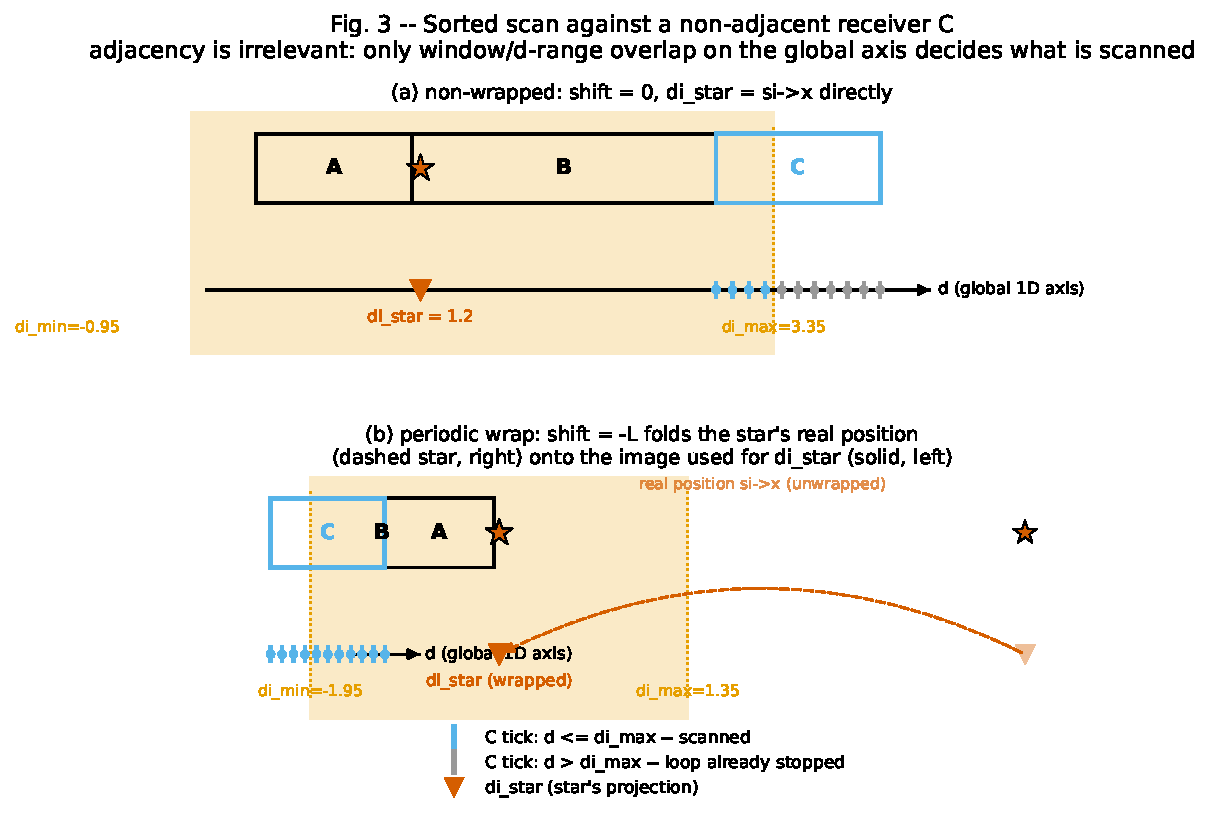
\includegraphics[width=0.95\linewidth]{figures/fig3_sorted_scan_nonadjacent.pdf}
  \caption{Sorted scan against a non-adjacent receiver \texttt{C}. Sort
    entries and the star's projection $d_{i,\star}$ are coordinates on
    the same global axis, so only window/$d$-range overlap decides what
    is scanned. Worked example (panel a): star at $x=1.2$, \texttt{C}
    spanning $[3,4]$, $R = 2.1$, $\Delta = 0.05$ gives the window
    $[-0.95, 3.35]$: exactly \texttt{C}'s ticks below $3.35$ are
    scanned, without \texttt{A} and \texttt{C} sharing a face. Panel (b):
    under periodic wrap the star is shifted by $-\vec{s}$ onto the
    receiver's side before projecting.}
  \label{fig:sorted-nonadjacent}
\end{figure}

\textbf{Any axis is conservative.} A 1D projection never exceeds the 3D
distance, so every true neighbour within $R$ falls inside the window
along \emph{any} of the 13 axes; the exact $r^2 < R^2$ test decides
membership (Fig.~\ref{fig:any-axis}). Correctness is therefore
axis-independent, and the axis choice is purely a pruning-efficiency
knob. This licenses the full fallback ladder: prefer the carried sid,
else scan forward along \emph{any} axis the receiver happens to be
sorted along, else the naive $O(N)$ loop: each rung trades speed,
never completeness.

\begin{figure}
  \centering
  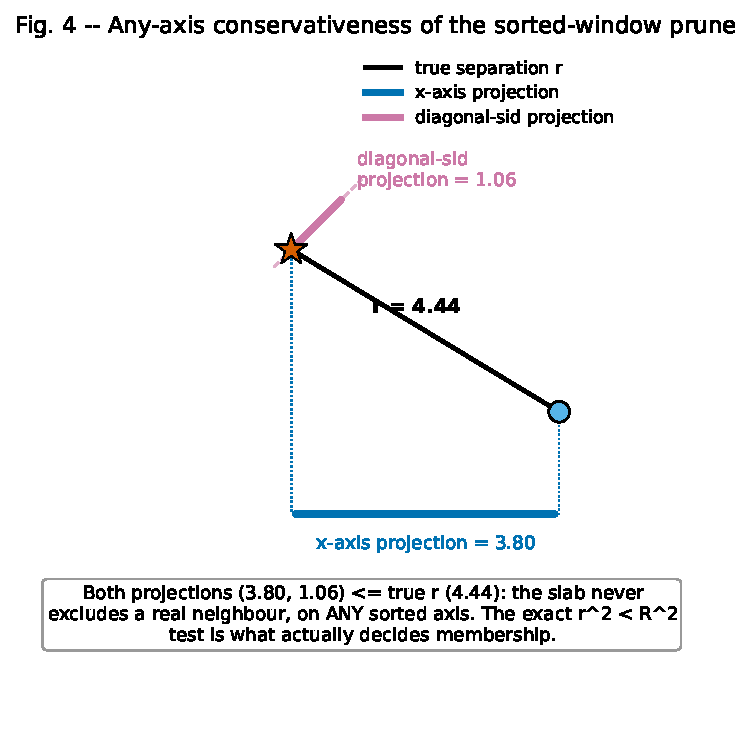
\includegraphics[width=0.75\linewidth]{figures/fig4_any_axis_conservative.pdf}
  \caption{Any-axis conservativeness of the slab pre-filter: both
    projections of the true separation are shorter than the separation
    itself, so the window admits a superset along any sorted axis and
    the exact $r^2$ test decides.}
  \label{fig:any-axis}
\end{figure}

\textbf{sid selection and its degradation bound.} The per-link sid is
chosen by per-axis \emph{sign} classification of the cell offset
(\code{runner\_hii\_visit\_neighbors}), not by direction matching: a
receiver offset by $(2,1,0)$ cell widths classifies as the $(1,1,0)$
edge axis. The projected separation then retains
$\cos\theta = 3/\sqrt{10} \approx 95\%$ of the true distance in that
example; the worst case over all lattice offsets (a long face offset
with unit transverse offsets, classified onto a corner axis) retains
$1/\sqrt{3} \approx 58\%$. The slab is thus never more than
$\sqrt{3}\times$ wider than the optimal-axis slab: a misaligned axis
costs extra exact-$r^2$ tests, never a missed neighbour, and the
cell-level window/$d$-range skip retains most of its selectivity even
along a poorly aligned axis. The same one-per-link sid is carried
unchanged down the receiver-side recursion, so off-axis leaves of a
large partner region are exactly where the any-axis fallback and the
exact test absorb the slack.

\textbf{Reach stays inside the wiring.} Sorting narrows the scan within
a visited cell; \emph{which} cells are visited remains governed by the
\code{radiation\_in} stencil of Section~\ref{sec:runtime}. The in-pass
radius-expansion loop is clamped to the reach the wired stencil
guarantees
(\code{max\_reachable\_search\_radius} in
\code{runner\_dosub\_stars\_hii\_ionization\_feedback}), so the sorted
machinery is never asked to find gas the task graph never wired; the
deferred outer shell is picked up after the next rebuild re-levels the
tasks.

\begin{figure}
  \centering
  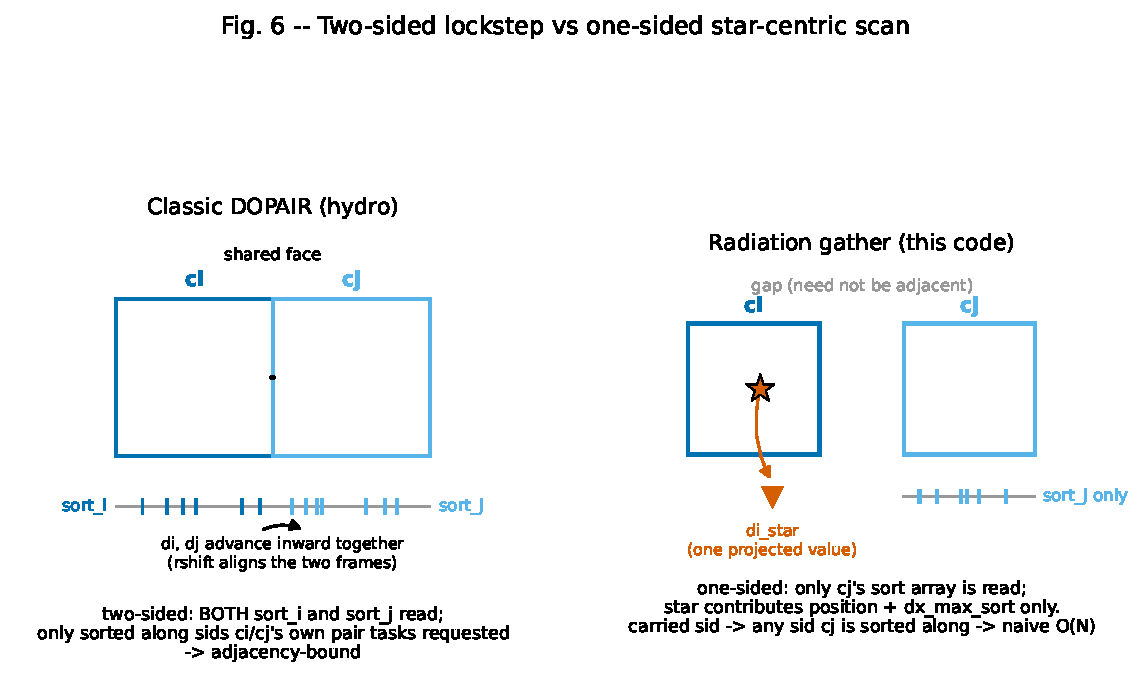
\includegraphics[width=0.95\linewidth]{figures/fig6_contrast_dopair_vs_radiation.pdf}
  \caption{Two-sided lockstep \texttt{DOPAIR} (adjacency-bound: both sort
    lists advance inward together along the pair's own axis) vs.\ the
    one-sided star-centric radiation gather (receiver's sorts only, one
    projected star coordinate, any-axis fallback). The one-sided form is
    what makes non-adjacent receivers unremarkable.}
  \label{fig:dopair-contrast}
\end{figure}

\textbf{The two-regions-away gap and its three guards.} When
\code{radiation\_level} sits at leaf level (no coarsening has happened
yet), the wired stencil of Section~\ref{sec:not-regular} is only a
leaf's up-to-26 immediate neighbours: a cell two regions away is not
filtered out, it is simply absent from \code{radiation\_in}, no edge
in the graph reaches it, even where the search radius geometrically
extends into it (Fig.~\ref{fig:stencil-gap}). Three guards bound how
far this gap can matter: (1) the split-gate equation of
Section~\ref{sec:not-regular} stops a region from splitting once its
own $h_{\rm hii}$ grows large enough, which coarsens
\code{radiation\_level} and folds the two-regions-away cell into the
now-larger wired stencil; (2) the radiation-specific rebuild check of
Section~\ref{sec:unskip} fires a whole-tree rebuild once the search
reach plus accumulated drift exceeds \code{dmin}, re-levelling the
stencil before the geometric gap can be exploited; (3) the in-pass
clamp above, \code{max\_reachable\_search\_radius}, stops a single
pass from probing past what the \emph{current} stencil can reach, so a
pass never silently drops a candidate it can see geometrically but
cannot walk to: the outer shell it cannot yet reach is deferred to the
next rebuild, never lost.

\begin{figure}
  \centering
  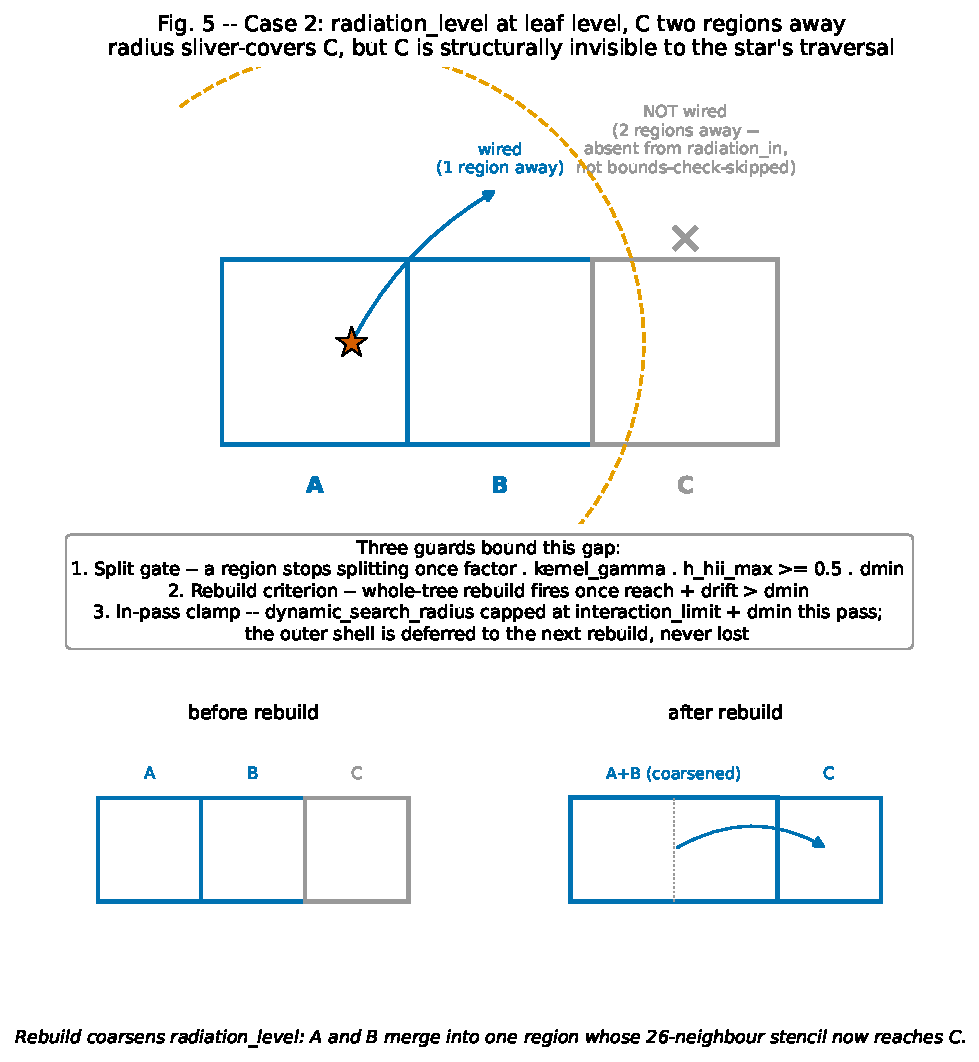
\includegraphics[width=0.85\linewidth]{figures/fig5_case2_stencil_gap.pdf}
  \caption{The two-regions-away gap: with \texttt{radiation\_level} at
    leaf level, cell C is two regions from the star and structurally
    absent from the wired stencil even though the search radius
    (dashed) geometrically reaches it. The three guards above bound
    the gap; a rebuild coarsens the stencil so C eventually enters it
    (before/after insets).}
  \label{fig:stencil-gap}
\end{figure}

\subsection{Cell sizing: folding \texttt{h\_hii} into \texttt{space\_regrid}}
\label{sec:space-regrid-hhii}

Everything above assumes the top-level cell grid is coarse enough that
a star's \code{radiation\_level} (Section~\ref{sec:not-regular}) can
actually reach every gas particle within its current \code{h\_hii}. That
grid is sized once per rebuild by \code{space\_regrid()}
(\code{src/space\_regrid.c}), which already folds ordinary hydro/star
\code{h\_max} into the top-level cell width: \code{h\_hii} was not
part of that calculation until this branch. Without it, a star whose
ionization search radius has grown large (in the fast-$Z=0$ growth
regime, the GEAR radiation logbook's Metallicity and the ionized-gas
temperature floor section, this can reach many pc) could in
principle out-grow a top-level cell grid sized only for ordinary
smoothing lengths, silently missing gas the search should have reached.

\code{space\_regrid()} now folds \code{c->stars.h\_hii\_max} (the
cell-aggregate, both the \code{local\_cells\_with\_particles\_top} and
\code{cells\_top} branches) and \code{s->sparts[k].h\_hii} (the
raw-particle fallback pass) into the same \code{h\_max} max-chain
already used for \code{hydro.h\_max}/\code{stars.h\_max}, so a star's
\code{h\_hii} can coarsen the top-level grid exactly like an ordinary
large smoothing length would.

\textbf{Why this needs a cap, not an unconditional fold.} Folding
\code{h\_hii} in unconditionally breaks the existing StromgrenSphere
acceptance example (the GEAR radiation logbook's Validation section),
which pins
\code{Scheduler:max\_top\_level\_cells: 3} with \code{periodic: 1},
already the hard minimum for periodicity (\code{cdim >= 3} per axis).
At \code{cdim == 3}, the 27-cell radiation stencil's $\pm1$ neighbour
wrap already covers every cell in the box, full coverage regardless of
how large \code{h\_hii} grows: a real Str\"omgren sphere reaching many
pc dwarfs a \code{cell\_min} sized for \code{dim/3}, so \code{h\_hii}
folded in unconditionally just pushes \code{cdim} below 3 and trips the
pre-existing ``must have at least 3 cells'' error. This is a
\emph{spurious} failure, not the missed-gas bug this change exists to
catch: there is nothing left to miss once periodic wrap already covers
the whole box.

\textbf{Fix: cap \texttt{h\_hii}'s own contribution to \texttt{h\_max}}
at the value that would size cells down to exactly \code{cdim == 3}
(\code{0.99 * dim\_min / (3 * kernel\_gamma * space\_stretch)}, the
\code{0.99} matching \code{space.c}'s own \code{tol} margin against
float-rounding at the boundary). \code{h\_hii} can still widen cells
(coarsen \code{cdim}) toward full coverage at finer starting
configurations (\code{cdim >= 4}, where \code{max\_top\_level\_cells}
is set higher); it just can never push \code{cdim} below the periodic
floor, since nothing is gained once coverage is already total there.
Ordinary hydro/star \code{h\_max} growth is \emph{not} capped: that
remains a genuine problem worth the existing error firing.

\textbf{Effect on \code{cdim}.} At the periodic floor
(\code{max\_top\_level\_cells: 3}, the StromgrenSphere acceptance
configuration above), the cap keeps the grid pinned at the correct
\code{cdim=3} throughout: with the fold left uncapped, the same run
instead crashes on the ``must have at least 3 cells'' error once
\code{h\_hii} grows large enough to push \code{cdim} below the
periodic floor, well before the box's true Str\"omgren radius is
reached. At a finer starting configuration
(\code{max\_top\_level\_cells} raised so the box starts at, say,
\code{cdim=16}, set by ordinary hydro resolution rather than the
radiation cap), the grid coarsens progressively as \code{h\_hii}
grows, passing through intermediate \code{cdim} values before settling
at \code{cdim=3} only once the fold's own cap requires it. This
progressive coarsening, not merely the crash-avoidance floor being
hit, is what confirms \code{h\_hii} is genuinely driving the grid
coarser to preserve radiation-search coverage.

\subsection{Configuration reference}
\label{sec:config-reference}

Every \code{Stars:}/\code{GEARFeedback:} identifier used above and in
the algorithm document is a parameter-file key, read with
\code{parser\_get\_opt\_param\_*} unless noted otherwise. All are
optional (default shown) except
\code{Stars:HII\_max\_search\_radius}, which every run using this
model must set explicitly.

\begin{center}
\small
\begin{tabular}{@{}p{5.6cm}p{1.5cm}p{7.6cm}@{}}
  \hline
  Parameter key & Default & Role \\
  \hline
  \code{GEARFeedback:with\_photoionization} & 0 & master enable switch \\
  \code{GEARFeedback:HII\_min\_density\_Hpcm3} & 1.0 & candidate density gate (algorithm doc, \S\ref{sec:photon-budget}) \\
  \code{GEARFeedback:HII\_max\_age\_Myr} & 50.0 & star age past which it stops competing for budget \\
  \code{GEARFeedback:HII\_rebuild\_time\_Myr} & 0.5 & per-star rebuild cadence (algorithm doc, \S\ref{sec:persistence}) \\
  \code{GEARFeedback:HII\_rebuild\_floor\_Myr} & $10^{-4}$ & floor on $\Delta t_{\rm back}$ (algorithm doc, \S\ref{sec:angular-splitting}) \\
  \code{GEARFeedback:HII\_deterministic\_boundary\_ionization} & 0 & boundary-particle rule (algorithm doc, \S\ref{sec:angular-splitting}) \\
  \code{GEARFeedback:HII\_angular\_nside} & 0 & angular pixel count (algorithm doc, \S\ref{sec:angular-splitting}) \\
  \code{GEARFeedback:HII\_couple\_ionization\_rate} & 0 & flag-and-floor vs.\ rate-coupled (algorithm doc, \S\ref{sec:rate-coupled}) \\
  \code{Stars:HII\_max\_search\_radius} & \emph{required} & hard ceiling on search-radius expansion (\S\ref{sec:runtime}) \\
  \code{Stars:HII\_max\_retry\_full\_buffer} & 10 & same-radius retry count (\S\ref{sec:runtime}) \\
  \code{Stars:HII\_max\_radius\_expansion\_tries} & 5 & radius-expansion retry count (\S\ref{sec:runtime}) \\
  \code{Stars:HII\_radius\_expansion\_factor} & 1.1 & radius growth per expansion (\S\ref{sec:runtime}) \\
  \code{Stars:min\_star\_timestep\_Myr} & $10^{-4}$ & generic star $dt$ floor, distinct from \code{HII\_rebuild\_floor\_Myr} \\
  \hline
\end{tabular}
\end{center}

One further knob is set at \code{./configure} time, not in the
parameter file: \code{--with-number-of-hii-angular-pixels} (default
12, i.e.\ $\text{nside}\le1$) sizes each star's per-pixel array and
bounds \code{GEARFeedback:HII\_angular\_nside} at runtime
(Section~\ref{sec:angular-splitting} of the algorithm document).
